% Copyright (C) 2010 Thomas L. Kula
% All Rights Reserved
%
% See the file LICENSE for license terms.
\documentclass[12pt]{article}
\usepackage{graphicx}
\usepackage{rotating}
\usepackage{fix-cm}
\setlength{\paperwidth}{5.5in}
\setlength{\paperheight}{8.5in}
\setlength{\textheight}{7.45in}
\setlength{\topmargin}{-1.0in}
\setlength{\oddsidemargin}{-0.5in}
\setlength{\evensidemargin}{-0.5in}
\setlength{\textwidth}{4.0in}
\setlength{\parindent}{0in}
\setlength{\parskip}{3mm}
\usepackage[print]{booklet} \nofiles
\source{\magstep0}{5.5in}{8.5in}
\target{\magstep0}{11in}{8.5in}
\setpdftargetpages
\pagestyle{empty}
\begin{document}


\begin{center}
{\fontsize{36}{48}\selectfont \textsc{Haiku a Day }}
\end{center}

\vspace*{3.5cm}

{\fontsize{20}{40}\selectfont 

At the last minute

One is forced to concentrate

And do the best work

}

\vspace*{5.0cm}
\begin{center}
{\large{Issue 60: June 2010}} \\[5mm]
{\fontsize{8}{8}\selectfont  \textsc{ St. Joshua Norton Press }} \\[1mm]
{\fontsize{6}{6}\selectfont Mathom House in Midtown \textbar The People's Republic of Ames }
\end{center}


\newpage

Back from Iowa, which was an amazing trip. Before any
of you read this, it will be time for Shadow Art Fair,
which I will have a table at with zines and photo prints.
In typical fashion, I'm scrambing around putting everything
together at the last minute, so until next month, enjoy.

--- Thomas

http://kula.tproa.net/had/ \\
kula@tproa.net

Download this and previous HADs at the website, so you can
print out your own (DIY, yeah!) or if you want me to send
you one, send me your address, and maybe a stamp if you
are feeling nice. Or send me something you've made ---
trades always appreciated, postcards are nice too.

\vspace*{2.5cm}

1 June 2010

Along the river \\
Grasses swaying in the breeze \\
Waving to the fish

2 June 2010

Hard and unyielding \\
Meets soft, sensative and tender \\
Staple in my foot

\newpage

3 June 2010

In the fridge, I'm scared \\
A collection of jars sits \\
Cold, empty, must clean

4 June 2010

I speak of bread, dense \\
Forged strong in a hot oven \\
Giving us true life

5 June 2010

From a box, a line \\
That Fibonacci's ratio \\
Installs the devine

6 June 2010

A malt at night sought --- \\
Who could make tasty drink? \\
Ice cream come to me

7 June 2010

Not time to awake! \\
Yet clearly there is the Sun. \\
Oh go fuck off, Sun.

8 June 2010

Sudden ice cream urge \\
Passes when something shiny \\
Discombobulates

9 June 2010

Ponderously swung \\
A door reveals a cavern \\
Vaporous with cold

\newpage

10 June 2010

The haste, in packing \\
Producing a small order \\
In a vast chaos

11 June 2010

Ten hours, a car \\
Music, coffee, and trail mix \\
I'm in Iowa

12 June 2010

The day a downpour \\
Growing calm, yet still muggy \\
And I'm in a suit

13 June 2010

Horay! Scooby Snacks. \\
A dish most devine arrives \\
Simple, tasty, good

14 June 2010

My old haunts I roam \\
They've changed, but still welcoming \\
I visit each one

15 June 2010

Lonely fried cheese ball \\
There a pool of ranch dressing \\
I drink some iced tea

16 June 2010

From Ames I depart \\
Off to Eastern Iowa \\
Before Michigan


\newpage

17 June 2010

A day filled with stamps, \\
Folding, knoting and tying \\
Makes invitations

18 June 2010

A long drive past me \\
At last in Ypsilanti \\
Gone fun, home better

19 June 2010

Waiting to return \\
Humidity makes horrid \\
All being outside

20 June 2010

There is confusion \\
When one thinks about the world \\
Fixing that is life

21 June 2010

The bathroom, now clean \\
After an hour of work. \\
Good for months now, right?

22 June 2010

Boxes, all my life \\
Putting things in other things \\
Striving for order

23 June 2010

A graveyard, my car \\
The shells of many things there \\
Waiting for cleaning


\newpage

24 June 2010

The cut of mustard \\
Burning a hole in my head \\
Strong yet flavorful

25 June 2010

More running, scrambling \\
Readying for tomorrow \\
Make a list, check it

26 June 2010

Seven, coming out \\
Gather food in the hundreds \\
Pedal for others

27 June 2010

Growing grey, the skies \\
Opening tormenting us \\
Rain flies, falls and fades

28 June 2010

Normally silent \\
Now you cry out as you bend \\
This hinge, annoying

29 June 2010

A deep growl rings out \\
Sputtering, coughing, unwell \\
My car is crappy

30 June 2010

This knot, confounding \\
An ache sits in my shoulder \\
Tying happiness


\newpage

\begin{center}
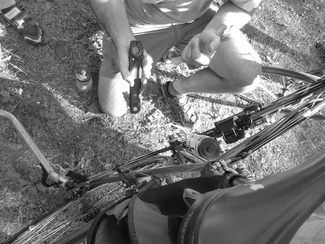
\includegraphics[width=4.25in]{cij.jpg} \\[1cm]

2010 Cranksgiving in June
\small{{\tt http://kula.tproa.net/photos/2010/2010-cranksgiving-in-june/ }}

\end{center}

\newpage

\thispagestyle{empty}
\vspace*{14cm}
\begin{sideways}
\Large{Thomas L. Kula}
\end{sideways}
\begin{sideways}
\Large{PO Box 980461}
\end{sideways}
\begin{sideways}
\Large{Ypsilanti MI 48198}
\end{sideways}


\end{document}


